\chapter{Introducción}
\section{Motivación del proyecto}

En el año 1994, tras una reunión en Sillicon Valley, Timothy C. May publica el manifiesto cripto-anarquista \cite{criptoanarquista} que da origen al movimiento Cyberpunk. Este movimiento social es el origen de una revolución de carácter libertaria cuyo principal objetivo es reducir la intervención del Estado a su mínima expresión. Se consideraba que la protección brindada por el Estado en la relación y acuerdos entre individuos, podía ser brindada de una manera más libertaria y eficiente por la tecnología. Dicho movimiento siembra las premisas de un proyecto que surge años después, el proyecto Bitcoin. \newline

El 1 de noviembre de 2008 se publica un artículo/White-paperXXXXXXX titulado “Bitcoin: A Peer-to-Peer Electronic Cash System” \cite{bitcoin}. El autor (o autores) del artículo/White-paperXXXXXX, que se esconde bajo el alias Satoshi Nakamoto, decide publicarlo en una lista de correo sobre criptografía. Este es uno de los primeros documentos en los que se menciona el término Blockchain. Se describe como una tecnología creada con el propósito de llevar a cabo el proyecto de Bitcoin. Blockchain surge de la ingeniosa combinación de distintas técnicas creadas años atrás en el campo de la informática y la criptografía. Apoyándose en los ideales del movimiento Cyberpunk, se describe al Bitcoin como una moneda digital gobernada por unas reglas criptográficas que controlan su gestión y emisión. La tecnología blockchain garantiza el correcto funcionamiento de los aspectos clave de las criptomonedas: la puesta en circulación de la moneda y el mecanismo de gasto que garantiza que una moneda no pueda ser gastada varias veces. Anteriores monedas digitales habían intentado resolver estos dos problemas sin éxito. El proyecto Bitcoin, cuya base tecnológica es blockchain, es la primera criptomoneda capaz de resolverlos de manera totalmente descentralizada. \newline

El problema del mecanismo para poner en circulación la moneda digital tiene su origen en el proyecto de Adam Back llamado HashCash. El proyecto tenía como objetivo combatir el correo spam haciendo uso de la técnica conocida como prueba de trabajo. La prueba de trabajo consiste en un problema matemático de resolución compleja pero cuya verificación es muy sencilla. El aspecto clave de la prueba de trabajo radica en que la dificultad del problema a resolver se puede ajustar. Es vital para cualquier moneda digital que la emisión de la misma sea predecible y constante en el tiempo. La regulación de la dificultad de la prueba de trabajo es el mecanismo por el cual se consigue ajustar la puesta en circulación. Las redes blockchain que hacen uso de la prueba de trabajo permiten que el usuario que antes resuelva uno de estos problemas emita (ponga en circulación) una determinada cantidad de nuevas monedas. El resto de usuarios de la red procederá a la sencilla verificación de la solución del problema antes de comenzar a buscar la solución a otro de estos problemas. \newline

Para resolver el segundo problema se necesita que los usuarios de la red sean capaces de conocer el último estado consensuado de la blockchain. Gracias a esto, los usuarios de la red serán capaces de determinar sin un usuario de la red es el poseedor de cierta moneda o no. En otras palabras, los usuarios de la red pueden verificar si un usuario en concreto está realizando un doble gasto de una determinada moneda o no. El trabajo del investigador Nick Szabo sobre la tolerancia a fallos bizantinos se convierte en la pieza clave para que los usuarios de la red lleguen al consenso sobre el último estado global de la blockchain. \newline

XXXXXXXXXXXXXTema 1 Alberto Toribio Intro a blockchain curso UNIR \newline

La tecnología blockchain permite a los usuarios de la red tener un registro válido, inalterable y consensuado de todas las transacciones realizadas. Los bloques de la cadena contienen la información relativa a esas transacciones, es por esto que a menudo se denomina a la blockchain como libro contable distribuido. \\
XXXXXXXXXXXXCambiar Ethereum a estado de la técnica????) \\
El 3 de enero de 2009 Satoshi Nakamoto crea el primer bloque de la cadena de Bitcoin conocido como bloque génesis. Desde ese momento se han estado creando nuevos bloques de la cadena y nuevos bitcoins ininterrumpidamente. Sin embargo, la popularidad de Bitcoin no ha sido la misma desde entonces. Durante los primeros años sufrió varios altibajos tanto en popularidad como en precio. Como se observa en la figura XXXXXXXX, no fue hasta finales de 2017 cuando su popularidad y precio comenzaron a incrementarse de manera exponencial. Entre 2009 y 2017 surgen muchas otras criptomonedas y proyectos basados en Bitcoin y blockchain.\newline

\begin{figure}
	\centering
	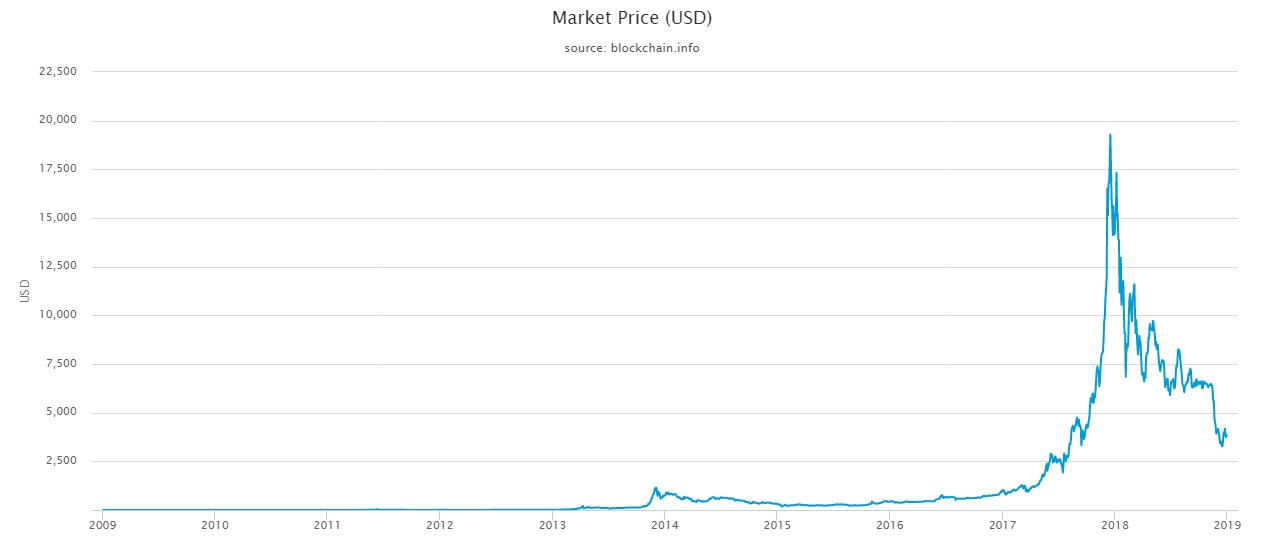
\includegraphics[width=1\textwidth]{imagenes/market-price-(usd).jpeg}
	\caption{\label{fig1}Precio Bitcoin \cite{blockchaininfo}.}
\end{figure}

El proyecto con mayor repercusión que hizo ver las posibilidades que ofrecía la tecnología blockchain más allá de Bitcoin fue Ethereum. El proyecto Ethereum, bajo el liderazgo de Vitalik Buterin, surge en 2014 con el objetivo de crear una nueva red blockchain. La red Ethereum, además de registrar todas las transacciones de su propia moneda digital (el Ether), registra pequeños programas informáticos llamados Smart Contracts. Los usuarios de la red, además de estar de acuerdo en las transacciones que se realizan en la red, deben estar de acuerdo en los despliegues de los Smart Contracts y de los resultados de la ejecución de los mismos. Con los resultados de la ejecución de los Smart Contracts ocurre exactamente igual que con las transacciones de monedas, si la mayoría de la red está de acuerdo (hay consenso) el resultado pasa automáticamente a ser válido. \newline

El nombre de Smart Contract puede llevar a equivocación. Los Smart Contracts no extienden todas las capacidades o características de un contrato convencional. Son programas informáticos que permiten programar una serie de instrucciones máquina propias de su máquina virtual (Ethereum Virtual Machine, EVM) para interaccionar con los datos que residen en memoria. Por lo tanto, la clase de tareas que podrán realizar los Smart Contracts será muy limitada. \newline

Uno de los principales usos de los Smart Contracts es la creación de tokens. Un token es una unidad de valor que una organización crea para gobernar su modelo de negocio y dar más poder a sus usuarios para interactuar con sus productos, al tiempo que facilita la distribución y reparto de beneficios entre todos sus accionistas \cite{business}. El Smart Contract asociado a un determinado token será el encargado de programar el registro y la interacción que se tenga con el token en cuestión. En definitiva, se tendría un pequeño libro contable creado sobre un gran libro contable (la blockchain) [XXXXXtema 1 UNIR]. \newline

La tokenización de activos abre un gran abanico de posibilidades, siendo su mayor práctica las ICOs (Initial Coin Offering). Permite una nueva forma de financiación a nuevas empresas. Consiste en la preventa de su propia moneda digital o token en representación de los servicios que dicha empresa prestará en el futuro. En el 2017 la financiación obtenida por empresas que han realizado esta oferta inicial de moneda supera los 5000 millones de euros [XXXXXbuscar dato real]. \newline

Tras toda esta serie de puntos de inflexión que han marcado el avance de la tecnología blockchain, es necesario citar los principales problemas, aún por resolver, entre los cuales se encuentra la principal motivación de este trabajo. \newline

La raíz de la mayoría de problemas está en la prueba de trabajo. La dificultad de los problemas de la prueba de trabajo se ajusta constantemente para hacer que el tiempo que empleará el poder computacional de todos los usuarios de la red en resolver el problema sea constante. Este tiempo tiene que ser suficiente para que la solución al problema hallada por un usuario sea difundida a la mayoría de usuarios y se adquiera el consenso. Este tiempo dependerá de las características de la red blockchain en cuestión. Cada solución a un problema permite que se añada un nuevo bloque a la cadena que contendrá la información relacionada con las transacciones realizadas. Cada bloque tiene un tamaño máximo que dependerá de cada red blockchain. Se tendrá por tanto un tiempo de creación y un tamaño máximo prefijado. Esto se traduce en una tasa máxima de transacciones por segundo (tx/s) para cada blockchain. Notar que la dificultad de la prueba de trabajo se ajusta en base al poder computacional agregado de todos los usuarios para que el tiempo sea constante. Esto significa que no por añadir más poder computacional a la red se incrementará el número de transacciones por segundo. Se observa en la figura XXXXXXXx como la dificultad de la prueba de trabajo de Bitcoin ha ido aumentando en el tiempo de manera similar a su precio y popularidad. Esto se debe a que conforme crecía el interés por la criptomoneda se incrementaba el poder de cómputo proporcionado por los usuarios a la red.\newline

\begin{figure}
	\centering
	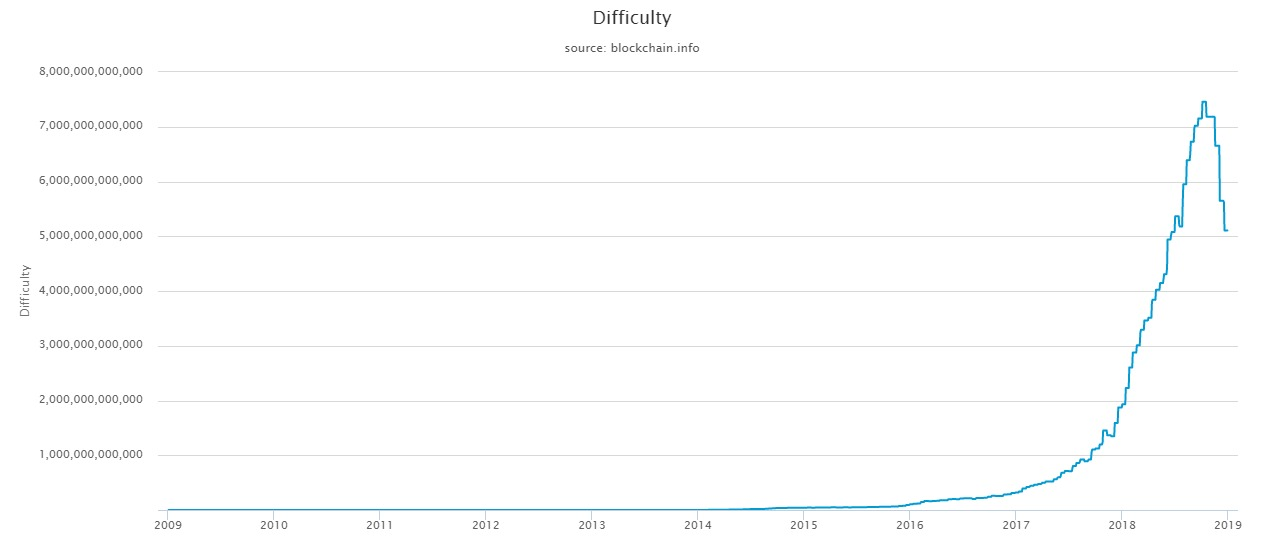
\includegraphics[width=1\textwidth]{imagenes/difficulty.jpeg}
	\caption{\label{fig1}Dificultad de la prueba de trabajo Bitcoin \cite{blockchaininfo}.}
\end{figure}

En la figura XXXXXXXX se observan el número de transacciones confirmadas por día entre 2017 y 2019, años en los que se observa el mayor incremento en la dificultad de la prueba de trabajo. Este incremento de poder de cómputo (traducido en incremento de la dificultad de la prueba de trabajo), no se traduce en un claro incremento en el número de transacciones por día.\newline

\begin{figure}
	\centering
	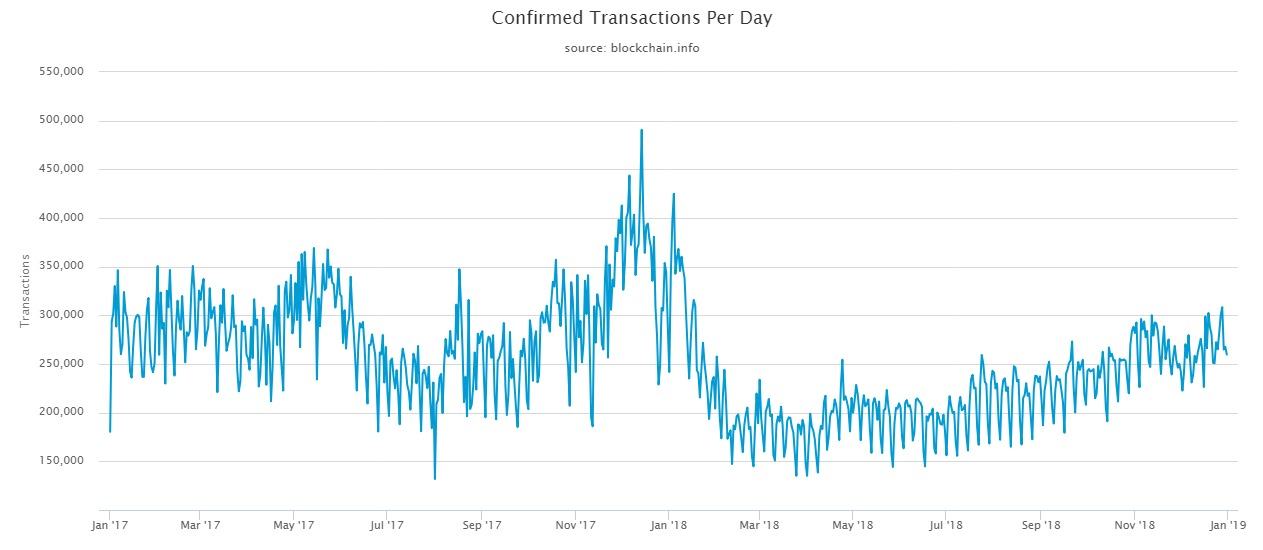
\includegraphics[width=1\textwidth]{imagenes/confirmed-transactions-per-day.jpeg}
	\caption{\label{fig1}Número de transacciones Bitcoin confirmadas por día \cite{blockchaininfo}.}
\end{figure}

Si un sistema no aumenta su rendimiento cuando se le añaden más recursos al mismo se dice de este que no es escalable. Es por esto que las redes blockchain basadas en prueba de trabajo son ineficientes por diseño. En base a la definición que se tiene, no se podrá conseguir que sea escalable como tal. Sin embargo, se podrán realizar cambios en el protocolo para hacer que sea lo más eficiente posible. Estos cambios en el protocolo que hagan que se consiga la máxima eficiencia posible están aún por descubrir y diseñar. \newline

La falta de escalabilidad da paso a otro de los principales problemas, el desperdicio de energía eléctrica. La reciente popularidad de las criptomonedas y las redes blockchain ha atraído el interés de muchas personas. Cada vez son más los usuarios que suman su poder computacional a la red con el objetivo de resolver los problemas de la prueba de trabajo. Sin embargo, el protocolo define que el tiempo empleado por el poder computacional agregado de todos los usuarios sea aproximadamente el mismo siempre. En otras palabras, si se aumenta el poder computacional de la red, aumentará también la dificultad de la prueba de trabajo para que entre todos tarden ese tiempo constante en resolverla. Este aumento de la dificultad se traducirá en un aumento de la energía eléctrica empleada en resolver la prueba de trabajo. El resultado siempre será la creación de un nuevo bloque de la cadena cada cierto intervalo de tiempo, la consecuencia directa que cuánto más poder computacional tenga la red, más energía eléctrica se empleará en el proceso. Existe mucha controversia acerca de si en realidad se trata de un desperdicio de energía eléctrica o no. Sin embargo, este debate no es el tema de este trabajo.
Cuando un usuario encuentra solución a la prueba de trabajo, este obtiene la capacidad de crear cierta cantidad de nuevas monedas que se autoasignará. Esto ha provocado la creación de grupos que aúnan todo su poder computacional en un mismo usuario para así aumentar la posibilidad de encontrar la solución a la prueba de trabajo recibir estas nuevas monedas creadas que posteriormente repartirán entre todos. Surge así un nuevo problema que atenta contra la descentralización de la red. En redes como la de Bitcoin, casi la totalidad de los nuevos bloques son incluidos a la cadena por tres de estos grupos como se observa en la figura XXXXXXXXXXXXXX. Se podría decir que estos tres grupos gobiernan la blockchain de Bitcoin. A esto se le suma que, si uno de estos grupos adquiere al menos el 51\% del poder computacional de la red, este podrá incluir las transacciones (válidas o inválidas) que desee a su antojo. Esto se conoce como el ataque del 51\% y es posible ya que este grupo haría que la mayoría de la red esté en consenso. En la figura XXXXXXXXXXXXXX se observa el porcentaje de éxito de cada uno de estos grupos durante el día 1 de enero de 2019. Notar que esta distribución se puede considerar constante durante el último año. \newline

La gran cantidad de inconvenientes aún por solventar o mejorar motivan este trabajo. En el siguiente apartado se definirá más concretamente el problema que se pretende atajar en el trabajo y los objetivos del mismo.\newline


\begin{figure}
	\centering
	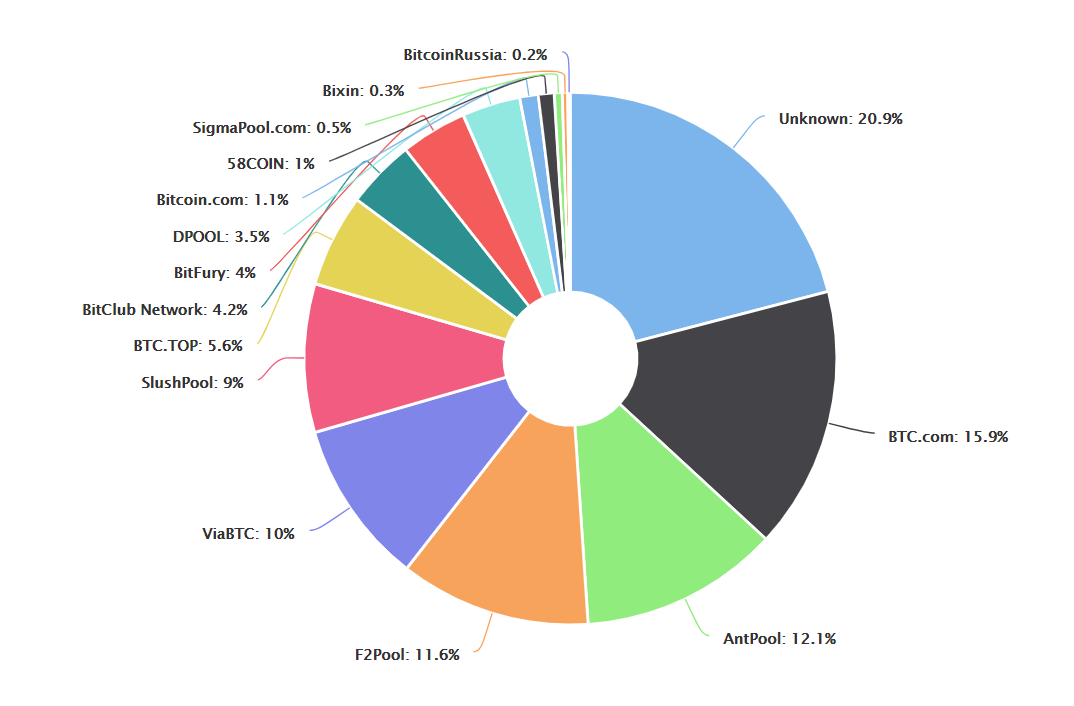
\includegraphics[width=1\textwidth]{imagenes/minninpools.PNG}
	\caption{\label{fig1}Porcentaje de pruebas de trabajo resueltas por cada grupo \cite{blockchaininfo}.}
\end{figure}





\section{Objetivos}

En el apartado ANTERIORXXXXXXXXXXXXXXXXXXX se describen los hitos más relevantes de la historia de las criptomonedas y blockchain. Una vez se conoce el porqué de su reciente popularidad se describen los problemas entre los cuales se encuentra la principal motivación de este trabajo. En este apartado se describirá con mayor detalle el problema que se pretende atajar en este trabajo y los objetivos del mismo. \newline

En base al protocolo actual que se tiene para las redes blockchain basadas en prueba de trabajo, ninguna de estas puede ser un sistema escalable. Si se quiere que una red blockchain basada en prueba de trabajo siga teniendo las características necesarias para sustentar una moneda digital, no se podrá conseguir que el sistema sea escalable como tal. Está diseñado para que sea ineficiente. Sin embargo, es posible hacer cambios en el protocolo para que, dentro de esa ineficiencia, el sistema sea lo más eficiente posible. \newline

¿Por qué está diseñado para ser ineficiente? La prueba de trabajo plantea problemas matemáticos a toda la red de usuarios de manera que el primero en encontrar la solución, la distribuya, sea el creador del siguiente bloque de la cadena y se lleve una recompensa por ello. El problema está en la distribución de la solución. Se necesita que la mayoría de la red esté de acuerdo con que un usuario en concreto ha sido el primero en encontrar la solución a la prueba de trabajo y todo lo que ello acarrea. El consenso debe llegar antes de que los usuarios de la red comiencen a buscar solución a la nueva prueba de trabajo. Los usuarios forman una red P2P, por lo que la distribución de la solución llevará su tiempo antes de que la mayoría de la red alcance el consenso. Para este tiempo es para el que se ajusta la dificultad de la prueba de trabajo, y no se puede reducir ya que sino la red no alcanzaría el consenso. En la red Bitcoin este tiempo es de aproximadamente 10 minutos. Suele ocurrir que, durante este tiempo de difusión de una solución, haya otros usuarios que, sin saber que alguien ya ha encontrado una solución, encuentren otra solución al mismo problema y comiencen a distribuirla desde otro punto de la red. Habrá usuarios de la red que reciban soluciones a la misma prueba de trabajo de distintos usuarios. Sólo una de ellas se puede considerar válida, y los usuarios deben ponerse de acuerdo en cuál de ellas. Cada vez que se encuentra una solución a la prueba de trabajo, a su vez se genera una nueva prueba de trabajo relacionada con esa solución anterior. El protocolo actual dicta que cuando un usuario recibe varias soluciones válidas a una misma prueba de trabajo, este debe elegir una de estas soluciones al azar y comenzar a buscar solución a la nueva prueba de trabajo generada. Cada usuario espera que la mayoría de la red haya elegido la misma solución que él, ya que sino estará buscando solución a una nueva prueba de trabajo distinta a la de la mayoría de la red y por ende inválida. Cuantas más soluciones se encuentren a la misma prueba de trabajo, más difícil resultará alcanzar el consenso. Por lo tanto, la dificultad de la prueba de trabajo se ajustará para que el número de soluciones concurrentes sea el mínimo posible.
A priori se puede pensar que resultaría mucho más eficiente que cada usuario sellara temporalmente su solución. Así cuando otro usuario de la red tenga que elegir entre varias soluciones, podrá hacerlo en base al sello temporal y no por azar. Esto da pie a otro de los puntos clave de las redes blockchain, y es que, al tratarse de redes P2P públicas, ningún usuario debe confiar en ningún otro. Por lo tanto, hay dos aspectos de los que ningún usuario debe fiarse:
\begin{enumerate}
	\item No se tiene la certeza de que otro usuario selle temporalmente una solución con la hora real de su reloj. Podría hacerlo con una hora previa para sacar ventaja de ello.
	\item No se tiene la certeza de que la hora real que marque el reloj de un usuario esté sincronizada con la hora UTC.
\end{enumerate}
	
El objetivo del presente trabajo consiste en solventar estos dos puntos. De conseguirlo, se podría hacer uso de un sellado temporal distribuido y confiable para las distintas soluciones que se encuentren a la prueba de trabajo. Se considera que esto permitiría a los usuarios de la red encontrar el consenso de manera más eficiente. Así se podría reducir la dificultad de la prueba de trabajo, sin que esto afecte al consenso, lo que supondría una mejora en el número de transacciones por segundo.


\section{Materiales y métodos}

\section{Organización de la memoria}